\documentclass[12pt]{article}

\usepackage[utf8]{inputenc}
\usepackage[T1]{fontenc}
\usepackage[french]{babel}
\usepackage[hidelinks]{hyperref}
\usepackage{graphicx}
\usepackage{amsmath}
\usepackage[linesnumbered,ruled,french,onelanguage]{algorithm2e}
\usepackage{listings}
\usepackage{subfigure}


\title{Rapport de Projet\\
Interpréteur de Système de Lindenmayer}
\author{Étudiants : \\ Boubacar Sadio DIALLO\\Damien MARIS\\Evens ANTOINE\\Manix-Emmanuel BIDUAYA MBUYI}
\date{26 Avril 2023}

\begin{document}
\maketitle
\thispagestyle{empty}
\newpage
\clearpage
\pagenumbering{arabic}


\tableofcontents
\newpage
\begin{figure}[htpb]
	\center
	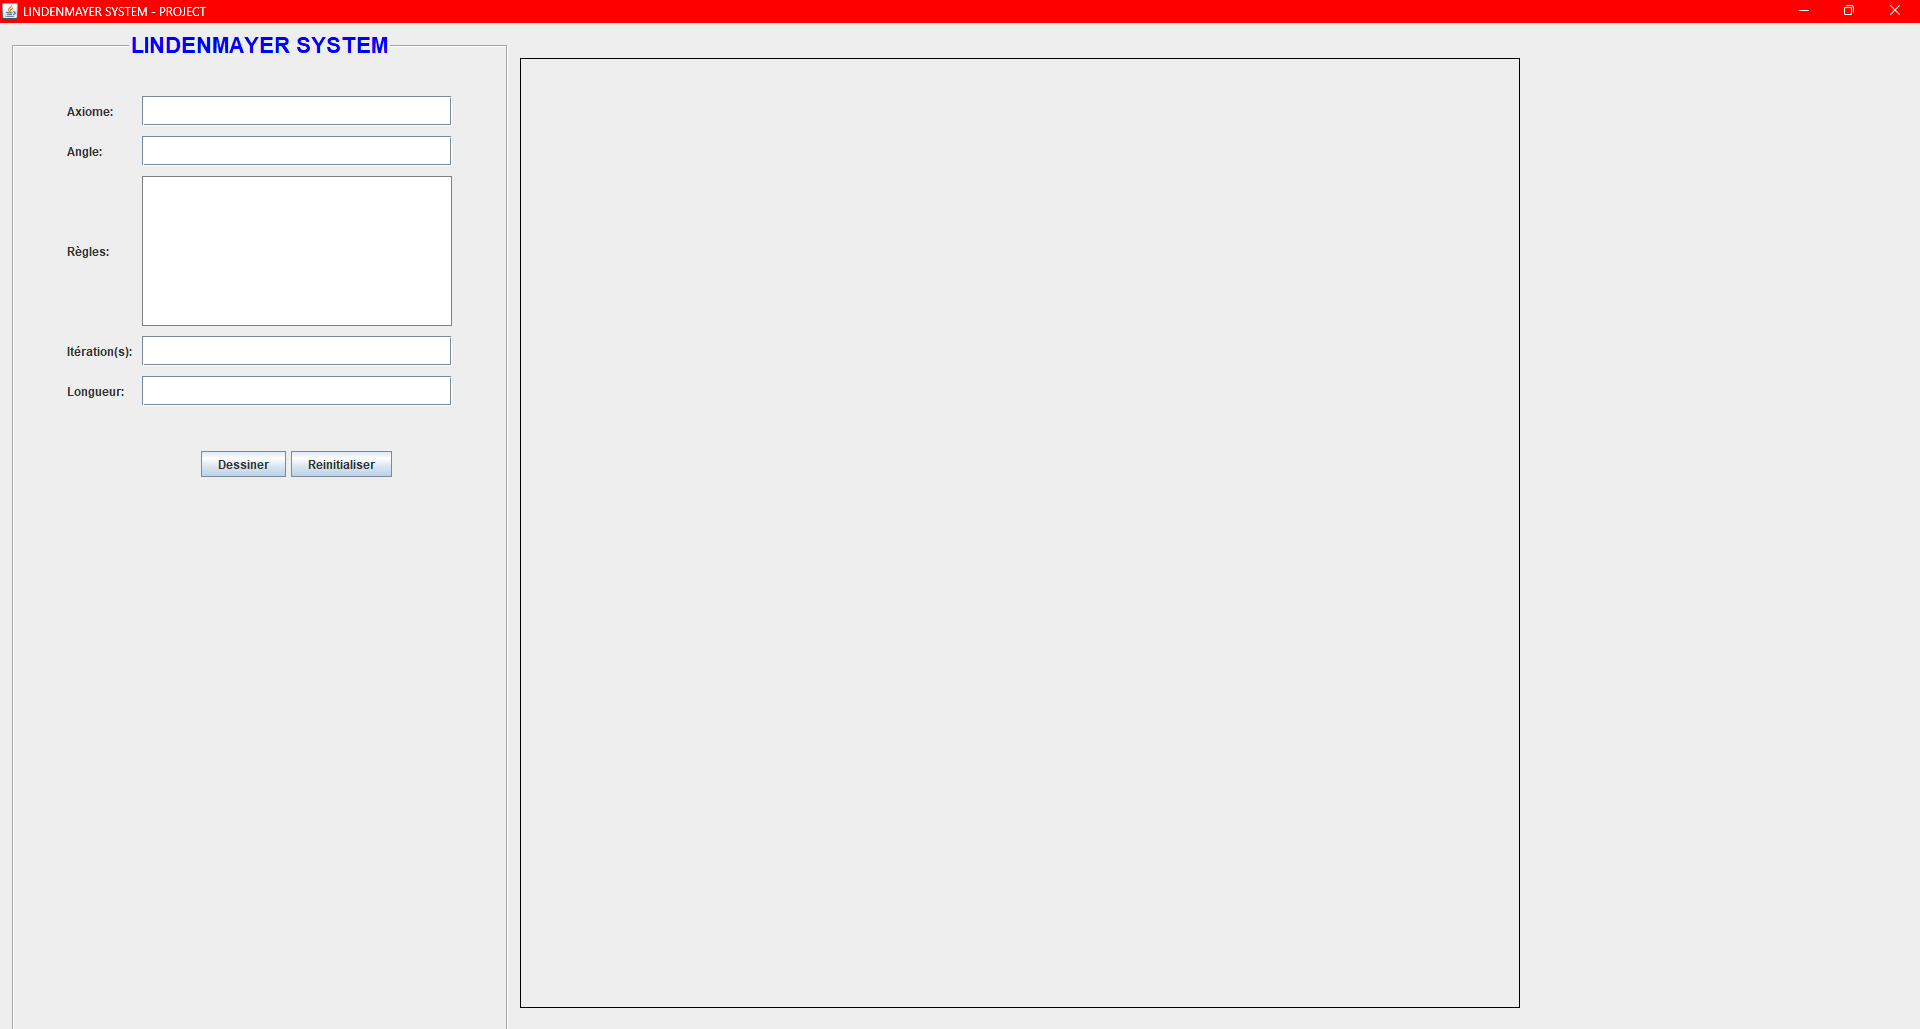
\includegraphics[width=1\textwidth]{./images/LSystemVide.png}
	\caption{LSystem blanc\label{fig:figure1}}
\end{figure}

\section{Introduction}
\subsection{Description générale du projet}
Le projet de L-System consiste en la conception et l'implémentation d'un programme capable de générer des fractales à partir de règles de substitution et de transformations géométriques. Ces fractales peuvent être utilisées pour modéliser des structures complexes plus ou moins réelles observées dans des jeux vidéo et des films d'animation, telles que les arbres, les plantes ou buissons. Ce système de réécriture permet également de créer des formes artistiques abstraites. Le projet comprend la conception et l'implémentation d'un système capable de traiter ces règles et transformations pour générer des arbres.

\subsection{Description générale de la problématique}
La problématique de ce projet est d'optimiser notre système de réécriture et d'interprétation, afin qu'il ne soit pas ni trop gourmand en ressource ni trop lent à l'exécution. Tout cela bien-sûr en respectant les dîtes contraintes imposées. Nous pouvons exposés quelques points durs qui sont les suivants : l'optimisation des complexités, le rendu graphique propre et cohérent et l'essai au mieux de garder une précision du dessin que l'interprétation va générer.

\subsection{Présentation du plan du rapport}
Nous allons donc bien évidemment parler de notre interpréteur de système-L. Le premier point que nous aborderons sera les objectifs du projet puis nous ferons un petit tour sur les quelques fonctionnalités que nous avons implémentées. Ensuite, quelques points techniques devront être évoqués. Puis nous nous dirigerons vers l'architecture du programme conçu. Enfin, avant de conclure ce rapport, nous vous exposerons quelques résultats de nos expérimentations.



\section{Objectifs du Projet}

\subsection{Description détaillée des objectifs et étapes majeures}
Le projet L-System avait pour objectif principal de concevoir et implémenter un programme capable de générer des arbres complexes à partir de règles de substitution et de transformations géométriques. Pour atteindre cet objectif, plusieurs étapes clés ont été nécessaires. Tout d'abord, on a commencé par définir l'axiome initial, qui est la base à partir de laquelle les arbres sont générés. Ensuite, on a fait la mise en place des règles de substitution permettant la transformation de l'axiome initial en des formes plus complexes à chaque itération du processus de génération. En outre, on a implémenté la tortue qui va interpréter chaque symbole de la chaine générée.
On implémente également le parser du L-System, qui est chargé de l'analyse syntaxique. Il permet de détecter si les symboles de l'axiome initial sont corrects, de vérifier si les règles de substitution sont bien écrites afin de déterminer les symboles à remplacer, ainsi que de gérer les itérations, l'angle et la longueur de déplacement de la tortue. 

\subsection{Description de travaux existants sur le même sujet}
Le système de Lindenmayer a été inventé en 1968 par Aristid Lindenmayer qui était biologiste. Ce système a été créé pour modéliser le processus de création des plantes. D'où la particularité de vouloir générer les dessins de flore. C'est donc au départ une étude botanique qui découla la théorie des L-Systems. Par la suite dans les années 1980, c'est Przemysław Prusinkiewicz, scientifique en informatique, qui en fait son principal sujet de travail. Certains ouvrages nous montre de nombreux exemples d'application de système de Lindenmayer. D'ailleurs, dans ce lien : \url{http://algorithmicbotany.org/papers/abop/abop.pdf}~\label{lien:lien1}, on y trouve beaucoup d'exemples de configuration de lsystem pour y afficher un arbre.




\section{Formalités implémentées}

\subsection{Description des fonctionnalités}

Grâce à notre projet nous vous proposons de manipuler un interpréteur simple de L-Système.
Notre projet propose donc une interface graphique permettant à la fois de configurer le L-Système ainsi que d'apercevoir le résultat. Notre logiciel vous demande d'entrer un axiome, un angle, des règles, un niveau d'itération ainsi qu'une longueur de trait.
L'axiome étant la graine de votre lsystem, c'est-à-dire l'itération 0, la base de la génération. C'est le point de départ de n'importe quelle récurrence.
L'angle demandé est celui qui déterminera l'angle de rotation des symboles \textbf{+} et \textbf{-}.
Les règles demandées sont les règles qui vont servir à obtenir une nouvelle génération en réécrivant les symboles.
L'itération est le nombre de niveau de génération que l'on veut effectuer.
Enfin, la longueur du trait détermine trivialement une longueur de trait.
Après l'entrée des règles, l'utilisateur est prié d'appuyer sur le bouton mis à disposition \textit{Dessiner}. Suite à ça le résultat sera affiché dans la fenêtre de droite.
Pour les vérifications, chaque zone de texte est soumis et analysé par un parser.
Si les champs sont valides, le résultat sous forme de chaine de caractères est copié dans le presse papier de l'utilisateur. Nous avons fait ce choix au lieu de l'afficher pour cause d'illisibilité.
Une méthode dans LSystem a été implémentée pour facilement transformer un String en une LinkedList de Symbole correspondant à chaque caractère du String.



\subsection{Organisation du projet}

Le projet a été réalisé en équipe, avec une répartition des tâches entre les 4 membres. Voici comment nous nous sommes partagés les tâches:
\begin{itemize}
	\item Manix-Emmanuel s’est occupé de la partie alphabet et caractérisation des symboles.
	\item Boubacar Sadio a réalisé la tortue et le parser.
	\item Damien a implémenté le LSystem, la gestion des règles et les tests.
	\item Evens a réalisé la partie graphique.
\end{itemize}

En plus de cette répartition, on a appliqué une méthodologie de développement en commun, avec des rencontres pour discuter de l'avancement du projet, de la structuration de ses différentes parties, de résoudre les problèmes et prendre des décisions collectives.



\section{Conception de langage}




\subsection{Interprétation des symboles}
Certains caractères du code ASCII, comme toutes les lettres de l'alphabet (majuscules et minuscules), nous servent comme représentation de symbole. Dans des classes représentant des symboles nous avons définis des ordres que nous fournissons à la tortue. Ces ordres vont être interprétés par la tortue. Et pour ce faire certains caractères sont attribués par défaut pour satisfaire les actions naturelles d'une tortue. En voici la liste :\\
\begin{itemize}
	\item \textbf{F} : Avance tout en dessinant
	\item \textbf{f} : Avance sans dessiner
	\item \textbf{-} : Tourne dans le sens horaire 
	\item \textbf{+} : Tourne dans le sens trigonométrique(anti-horaire)
	\item \textbf{[} : Sauvegarde la position actuelle
	\item \textbf{]} : Restaure la dernière position sauvegardée
	\item \textbf{|} : Tourne de 180°
	\item \textbf{\^} : Pointe la tortue vers le haut
	\item \textbf{\&} : Pointe la tortue vers le bas
	\item \textbf{<} : Pointe la tortue vers la gauche
	\item \textbf{>} : Pointe la tortue vers la droite
\end{itemize}

Tous ces symboles sont attitrés à un type de Symbole.

\subsection{Définition de l'axiome et règles de substitution}
Cette étape consiste à déterminer la séquence de symboles de départ qui est l'axiome initial à partir duquel la génération de l'arbre commencera, ainsi que de définir les règles de substitution qui indiquent comment les symboles seront remplacés par d'autres symboles ou séquences de symboles à chaque itération du processus de génération.
Voici un exemple de comment les règles doivent être écrites:
\begin{figure}[h]

$F=FF+$\\
$A=AB$\\
$-=-+$
\end{figure}




\section{Éléments techniques}
\subsection{Description des paquetages non standards utilisés}
Afin de tester certaines de nos classes, nous avons décider d'utiliser \textit{JUnit}, qui nous permet de faire des tests unitaires de façon plus efficace pour nos objets. En abordant cela, nous avons aussi fait le choix de créer des tests seulement sur les classes principales méritant un test. Ce sont les classes \textit{\textbf{LSystemTest}} et \textit{\textbf{ParserTest}}, qui sont explicitement les classes de test pour les classes \textit{\textbf{LSystem}} et \textit{\textbf{Parser}}.\\
Nous avons un package \textit{controller} qui contient les classes permettant la MVC de notre projet.

\subsection{Description des algorithmes (non triviaux)}
\subsubsection{LSystem}

Pour la configuration du LSystem, après la validation de la saisie des champs. Nous devons mettre à jour les règles de l'instance du LSystem. Pour cela nous utilisons l'algorithme~\ref{algo:algo1} suivant\\
\begin{algorithm}[H]
\DontPrintSemicolon
\SetAlgoLined
\KwIn{chaine de règles $chaineRules$}
\KwOut{mise à jour des règles du système L}
$chaqueRegle\gets$ tableau de chaînes créé en divisant $chaineRules$ en lignes en utilisant "\textbackslash n" comme séparateur\;
\For{$a$ dans $chaqueRegle$}{
\If{$a.length()!=0$}{
$this.lsystem.changerRegleSymbole(a.charAt(0),a.charAt(2))$\;
}
\If{$a.length()>3$}{
\For{$i$ de 3 à $a.length()-1$}{
$this.lsystem.ajoutRegleSymbole(a.charAt(0), a.charAt(i))$\;
}
}
}
\caption{MISE A JOUR REGLES\label{algo:algo1}}
\end{algorithm}
Dans cet algorithme, nous séparons les différentes règles différentiables grâce aux '\textbackslash n'. Pour mettre chaque règle dans une case d'un tableau de String. Puis, on va réécrire avec ce qui est donné les règles du symbole (celui devant le '=').

\subsection{Description des structures de données}
Nous avons fait le choix d'utiliser majoritairement les LinkedList<> quand nous avions besoin de stocker plusieurs symboles. Que ça soit pour la liste qui montre l'évolution du Symbole ou pour l'axiome du LSystem.
Pourquoi avons-nous choisi cela?
Et bien, nous pensons que c'est la structure de données la plus adaptée puisque à chacune des utilisations, nous parcourant tout le temps la liste du même sens et si nous voulons ajouter un élément, nous le faisons seulement en insérant à la fin de la liste.\\

Pour les positions de sauvegarde, dans la tortue, nous utilisons les piles et notamment la pile Stack fournie par Java.

Pour stocker les règles, nous utilisons une table de hachage fournie par Java, HashMap, où la clé est un Character, et la valeur est de type Symbole. 

\section{Architecture du projet}

\subsection{Diagramme des classes}
\begin{figure}[h]
	\center
	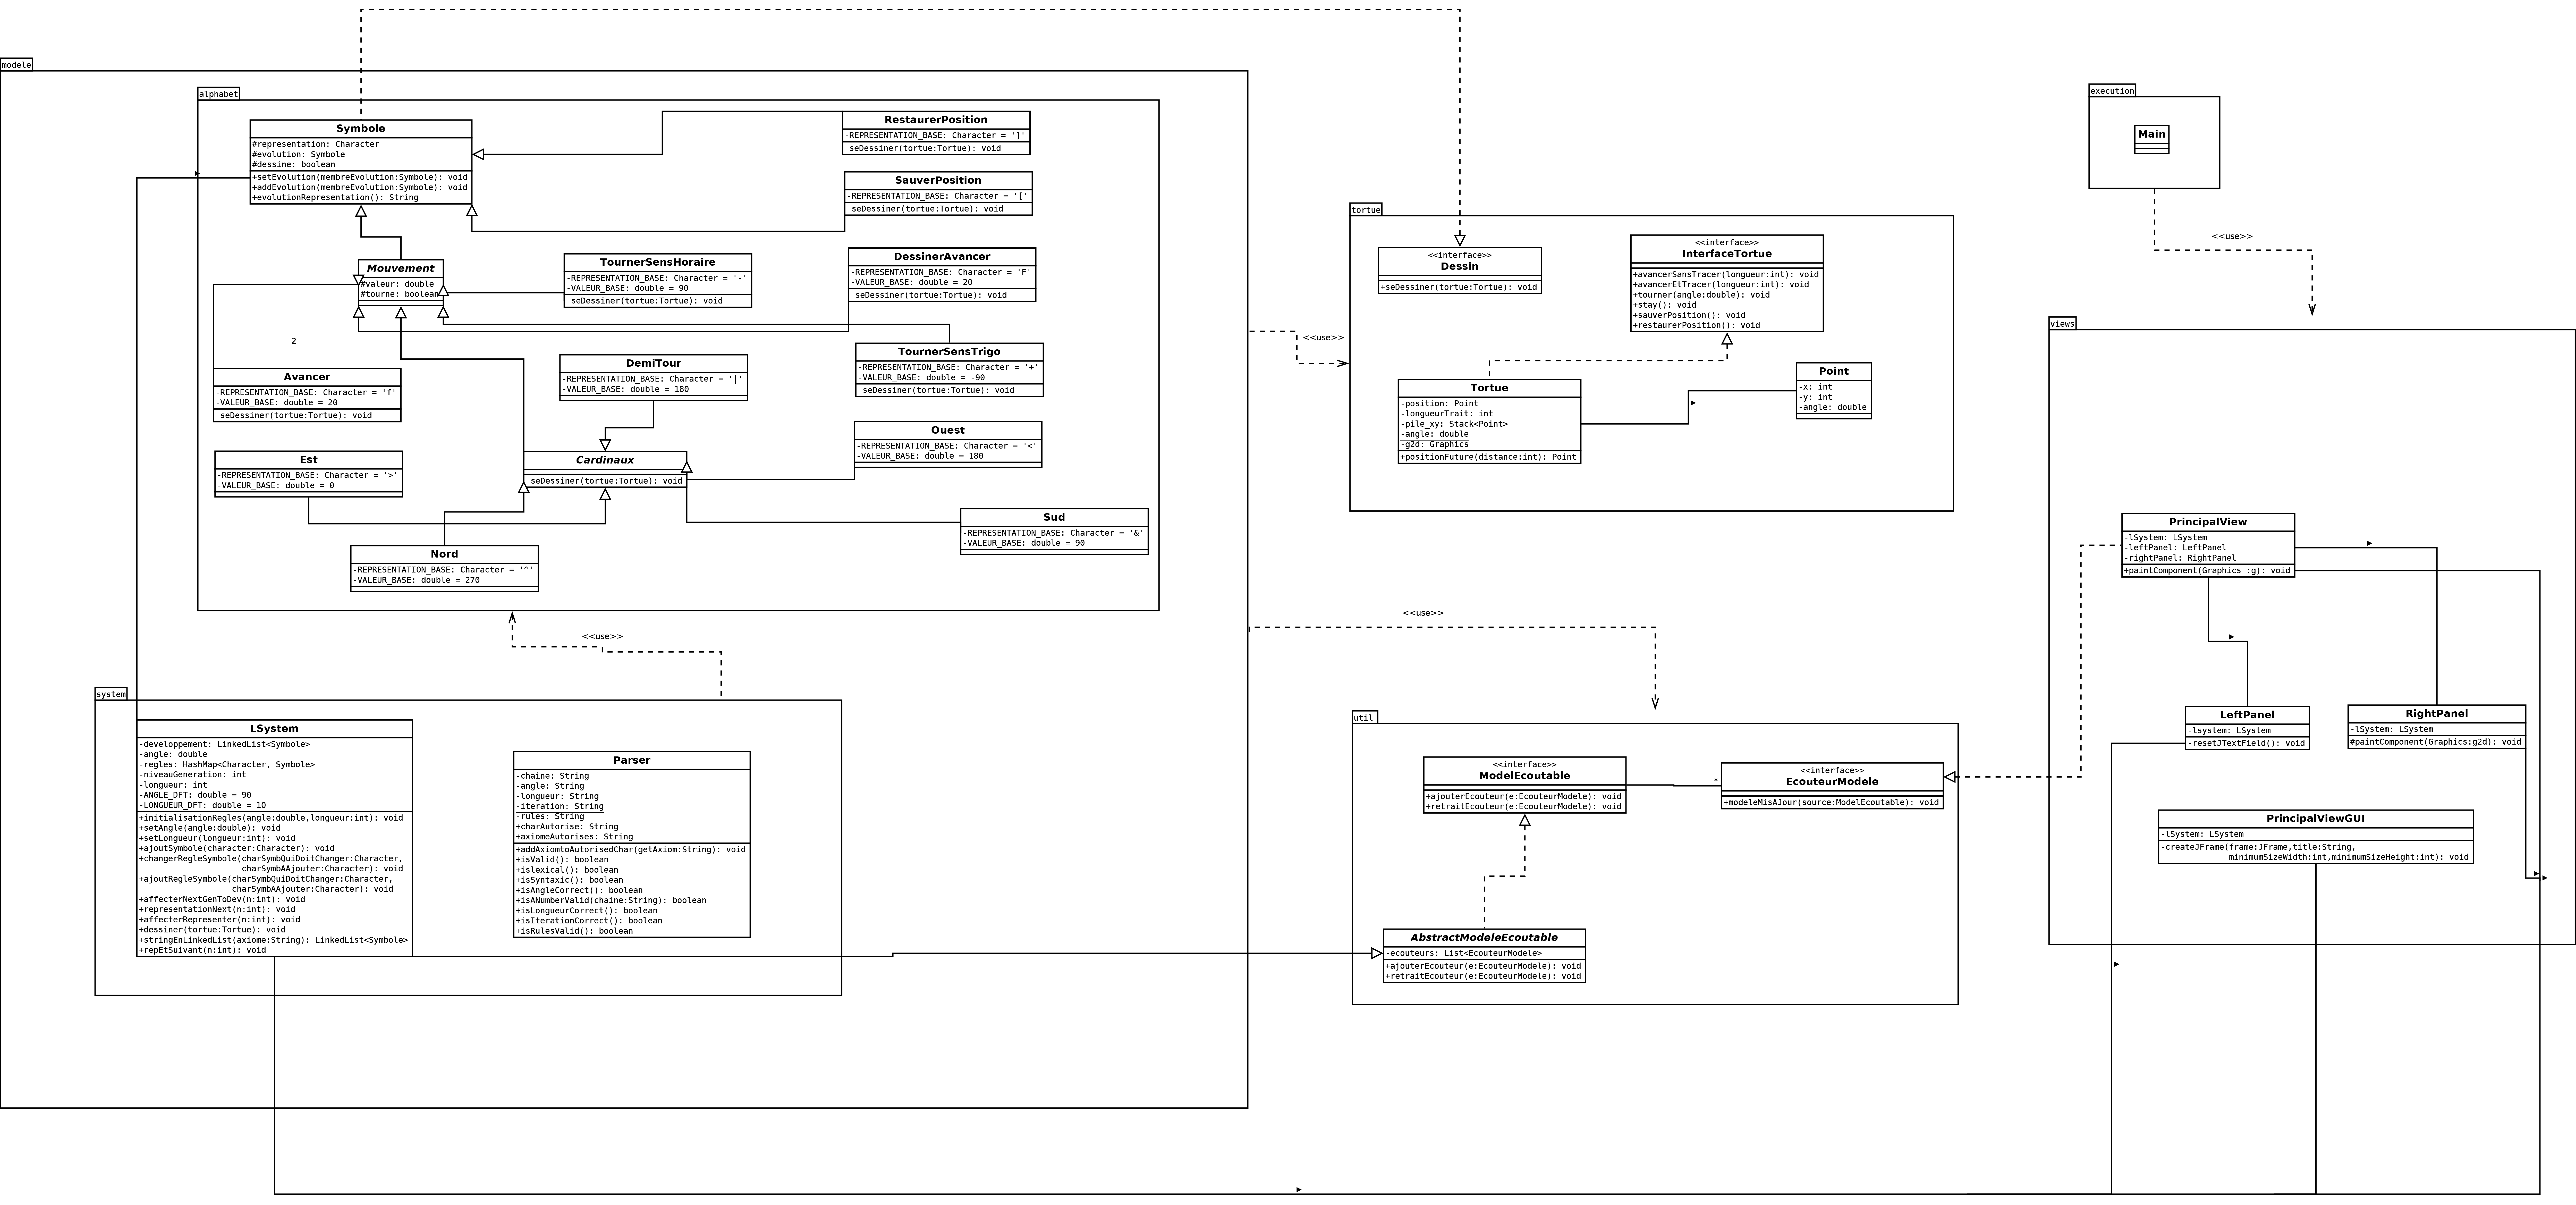
\includegraphics[width=1\textwidth]{./images/DiagrammeLSystem.png}
	\caption{Diagramme de classes du projet\label{fig:figure2}}
\end{figure}

Ci-dessus le diagramme des classes complets du projets. Par la suite, nous allons vous expliquer ce diagramme en vous expliquant en même temps l'arborescence des packages.

Le dossier \textit{src} possède 6 sous-packages qui sont :
\paragraph{execution}
Le package \textit{execution} contient la classe Main qui est la classe exécutable.
\paragraph{models} 
Le package \textit{models} qui est le package contenant tous les packages servant au modèle qui sont :
\subparagraph{alphabet}
Le package contenant toutes les classes dérivant de la classe Symbole
\subparagraph{system}
Le package contenant toutes les classes permettant d'établir les règles de déroulement d'un LSystem et d'établissement.
\paragraph{tests}
Le package \textit{tests} contient les classes de Test.
\paragraph{tortue}
Le package \textit{tortue} contient la classe Tortue et les classes servant à Tortue.
\paragraph{util}
Le package \textit{util} contient les classes du controller pour la MVC.
\paragraph{views}
Le package \textit{views} contient les classes servant au rendu graphique.
\begin{figure}[!h]
	\center
	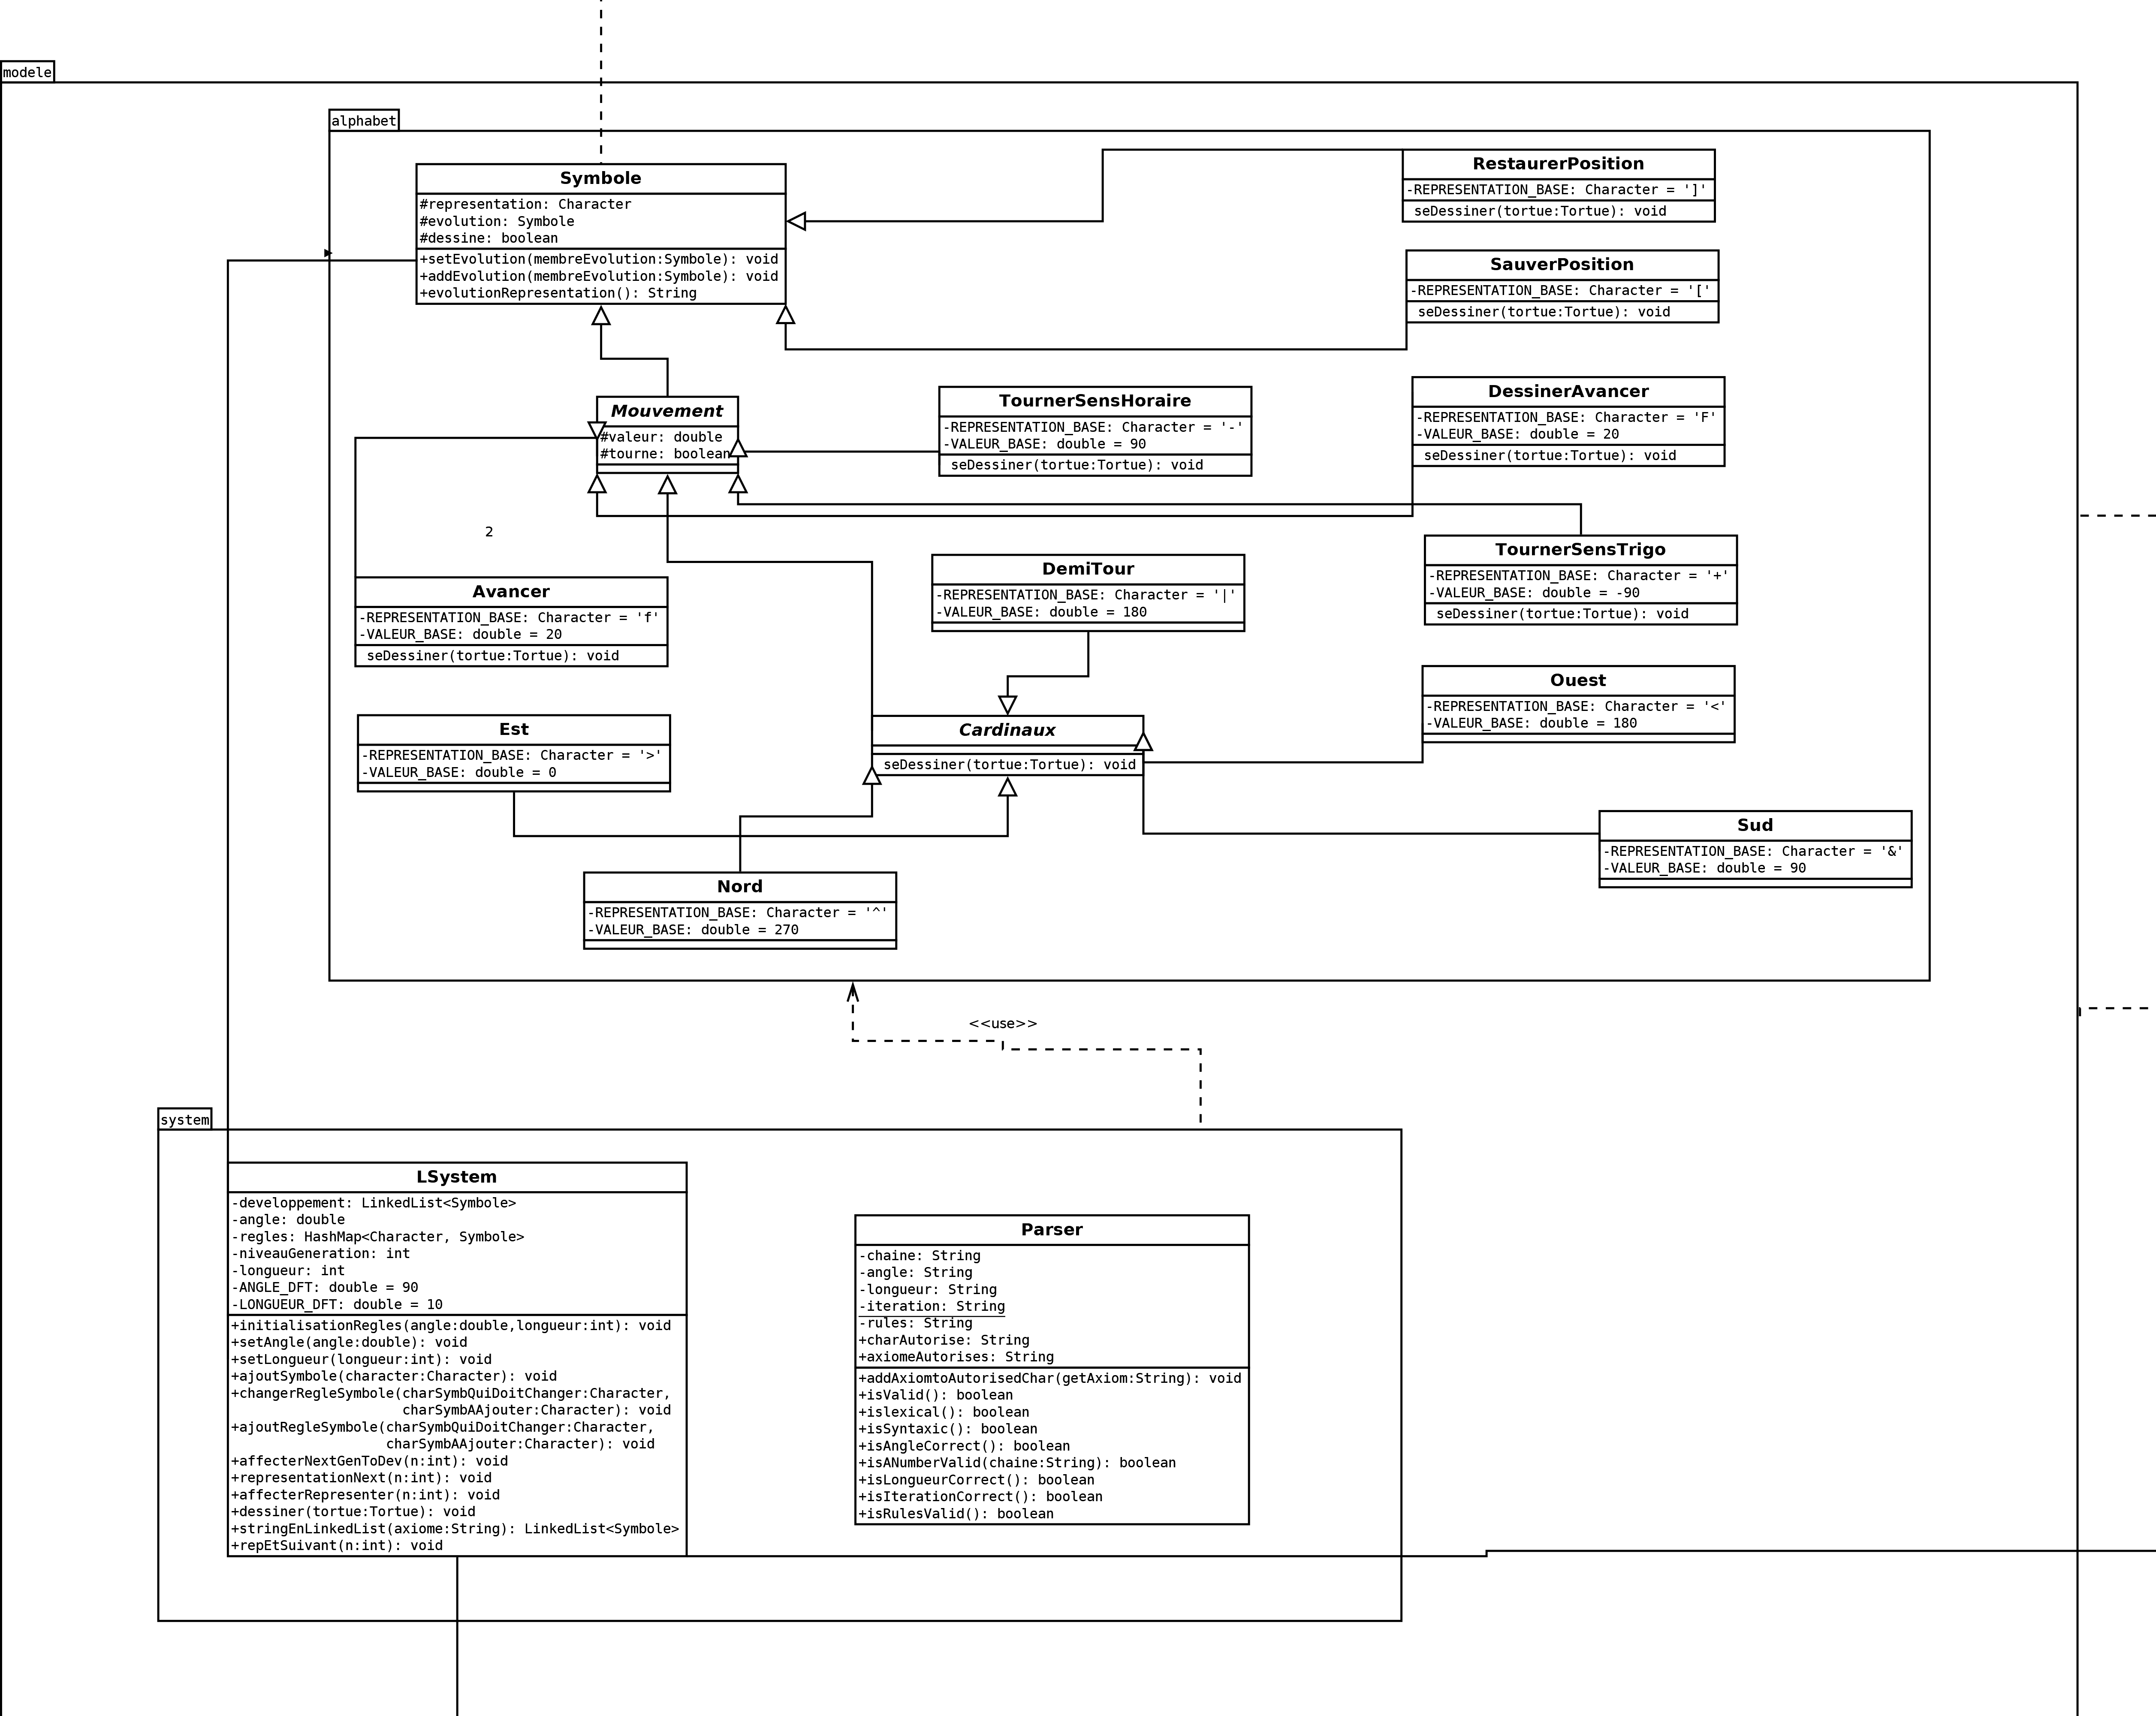
\includegraphics[width=0.8\textwidth]{./images/DiagrammeLSystemGauche.png}
	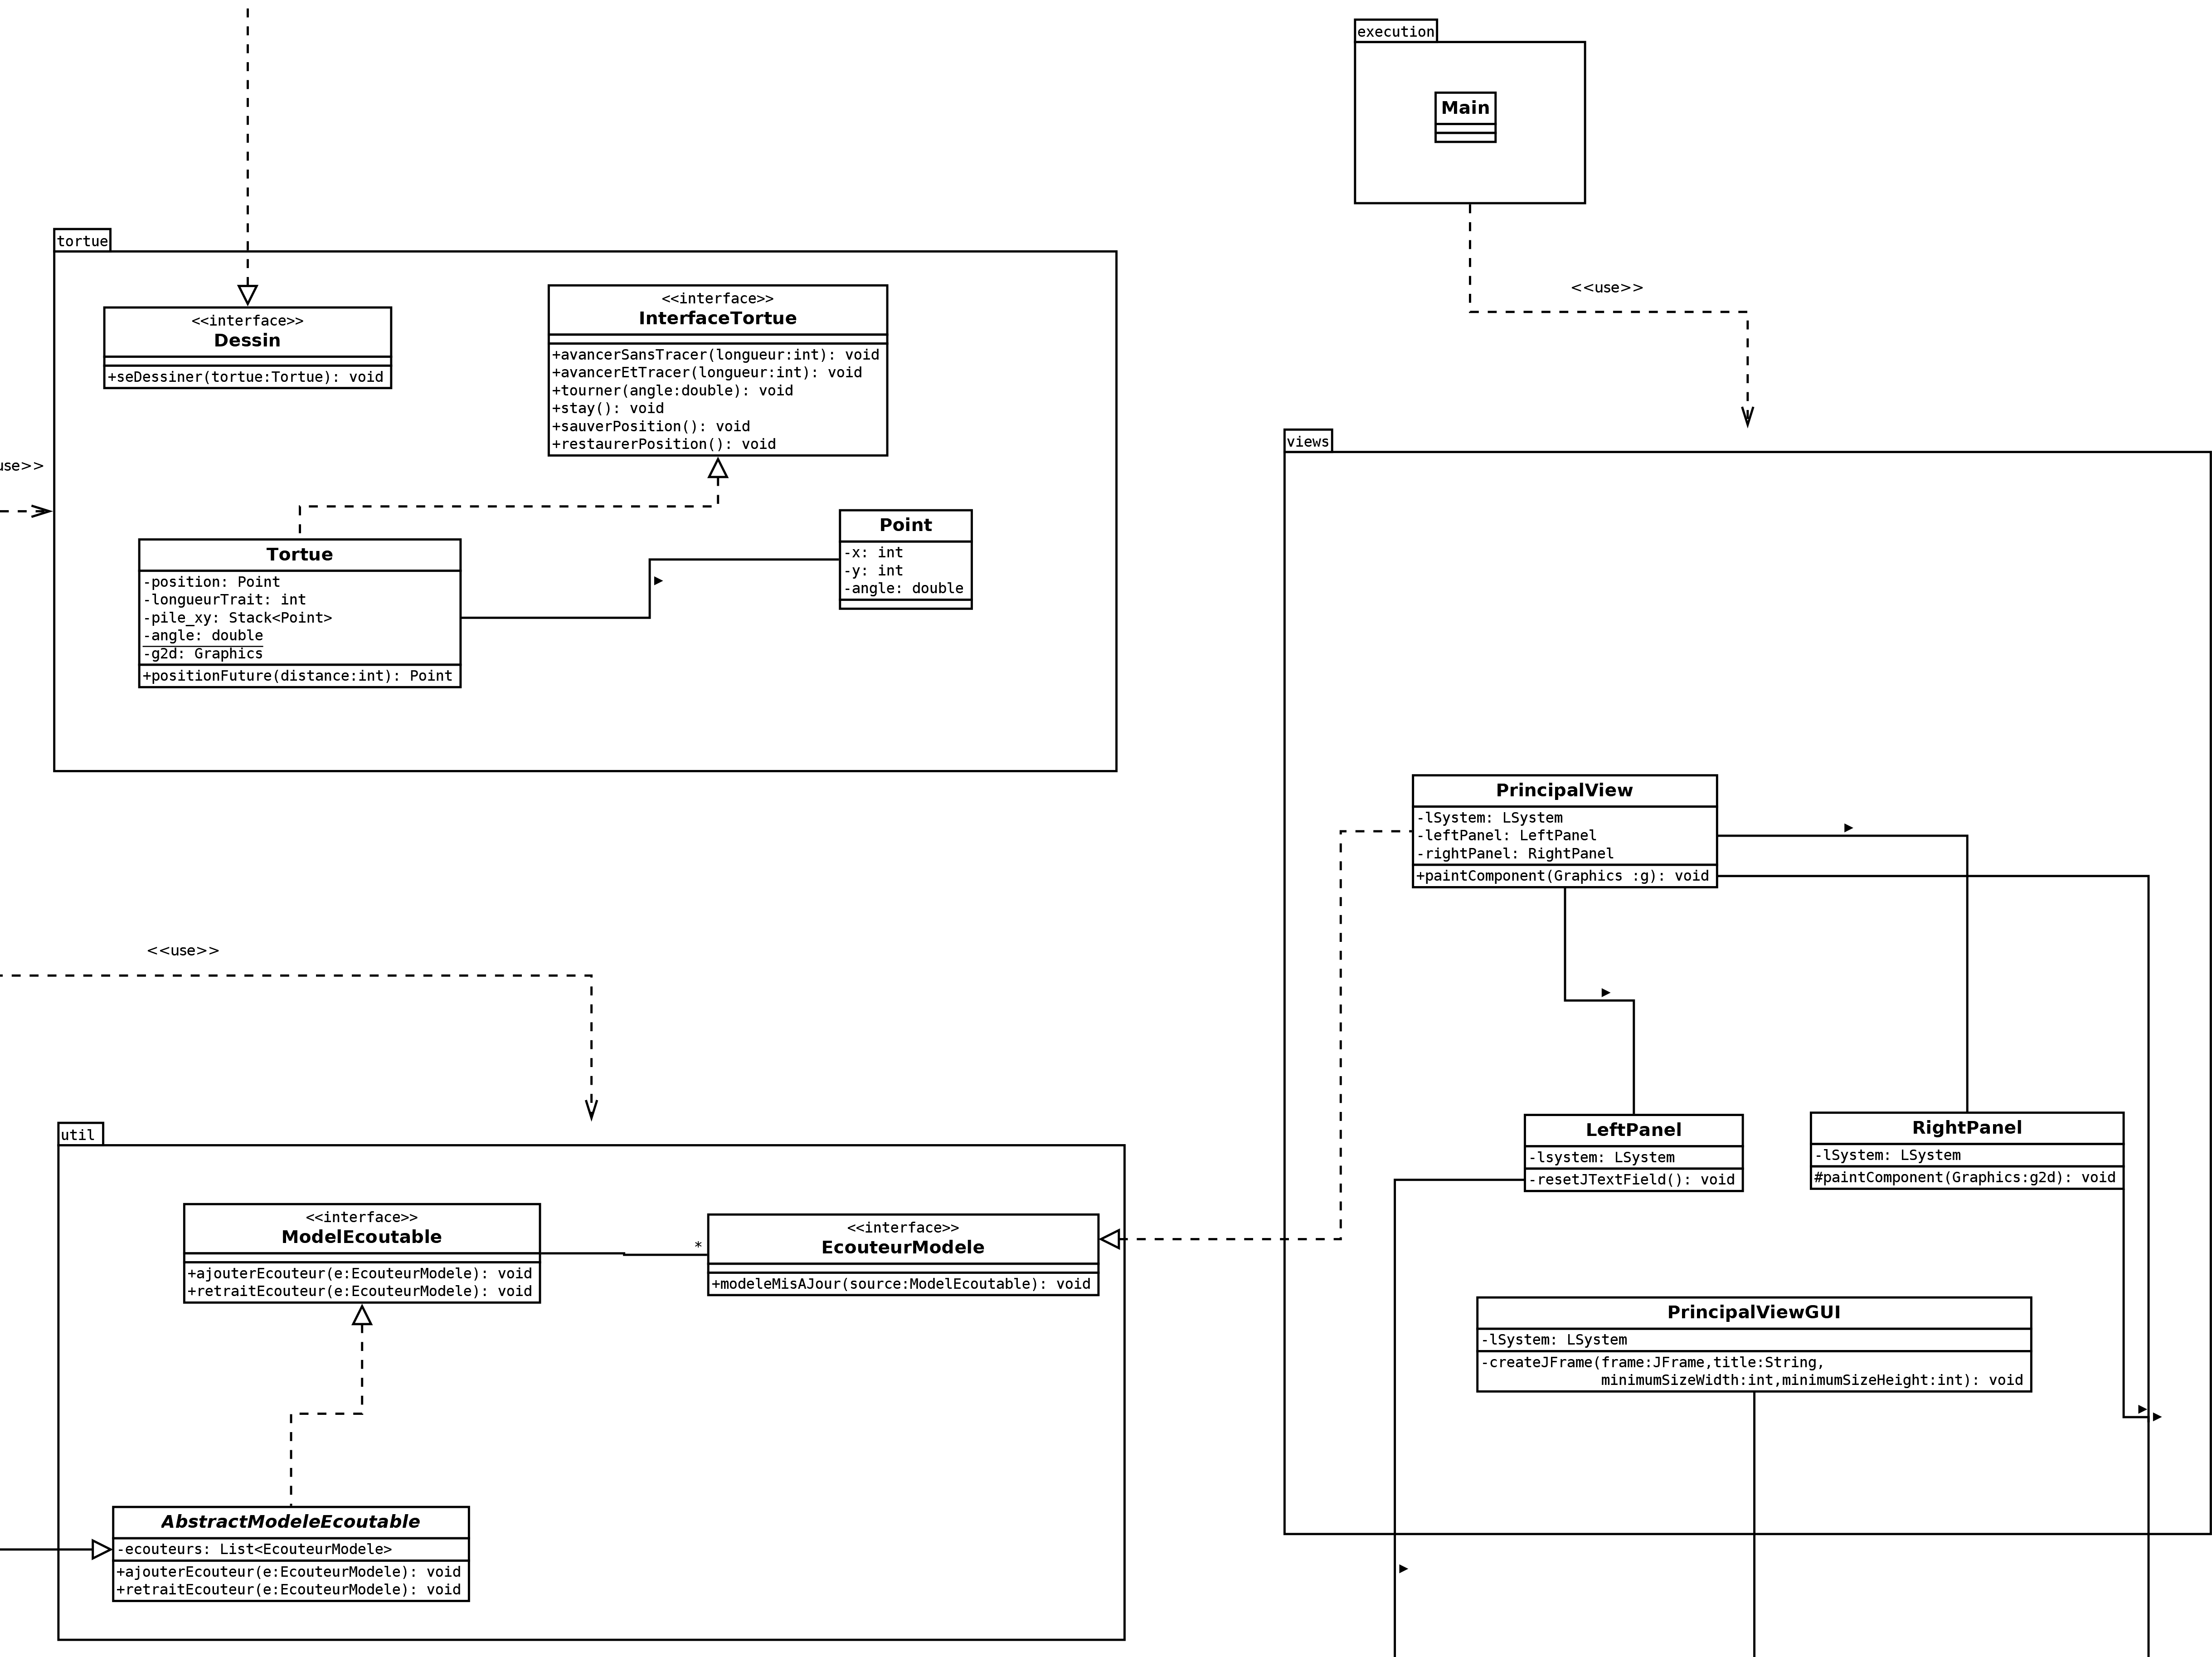
\includegraphics[width=0.8\textwidth]{./images/DiagrammeLSystemRight.png}
	\caption{Diagramme de classes zoom\label{fig:figure3}}
\end{figure}
 
\subsection{Chaînes de traitement}
Dans ce projet la classe majeure est la classe Symbole. Elle est la classe mère de nombreuses classes.
Un objet de classe Symbole possède un caractère en guise de représentation, sait s'il dessine et a une LinkedList de Symbole comme attribut. La classe Symbole sait donc se réécrire toute seule. C'est toute la force de notre structuration afin de satisfaire la partie réécriture d'un système-L.
Chaque classe contenu dans le package \textit{alphabet} hérite de Symbole.
Il existe dans ce package un autre niveau d'abstraction. Il y a la classe abstraite Mouvement (héritant bien-sûr de Symbole) qui ajoute comme attribut une valeur. Toutes les classes qui font la définition d'exercice d'un changement d'angle ou d'un changement de position héritent de la classe Mouvement.
Mais encore, il y a une autre classe abstraite intitulé Cardinaux qui font la définition de Symbole de rotation fixe dans les quatre points cardinaux de la fenêtre.

Tous ces symboles implémentent l'interface Dessin qui demande la redéfinition de la méthode :
\begin{lstlisting}[language=Java]
public void seDessiner(Tortue tortue);
\end{lstlisting}
, et chaque type de Symbole possède une redéfinition qui varie de celle des autres.
La seule classe pouvant dessiner est la classe \textbf{DessinerAvancer}.

\subsection{Fonctionnement}
Quand les champs sont validés, le lsystem est configuré en fonction de ce qui a été tapé.
Puis l'axiome va évoluer grâce à la méthode \begin{lstlisting}[language=Java]
public void affecterNextGenToDev(int n);
\end{lstlisting}
celle-ci va appeler une fonctionner qui va calculer le nouvel axiome et modifier l'ancien pour le remplacer par le nouveau.
\\
Comment l'axiome est-il calculé?
On va créer une LinkedList<Symbole> puis pour chaque Symbole de la LinkedList (grâce à un foreach) nous allons ajouter à la nouvelle LinkedList, la LinkedList caractérisant l'évolution du Symbole et ainsi de suite.

A la fin, de ce calcule, nous parcourons toute la liste afin d'obtenir les instructions qui vont permettre à la tortue d'évoluer et de nous rendre un dessin.
A chaque itération de boucle la Tortue comprend un ordre donné par le Symbole et exécute. La tortue utilise les méthodes de la bibliothèque Swing et y dessine dans un JPanel, jusqu'à que toute la liste ait été parcourue.

 
\section{Expérimentation et usages}
\subsection{Cas d'utilisation}
\begin{figure}[!ht]
\centering
\subfigure[Arbre en Fractal]{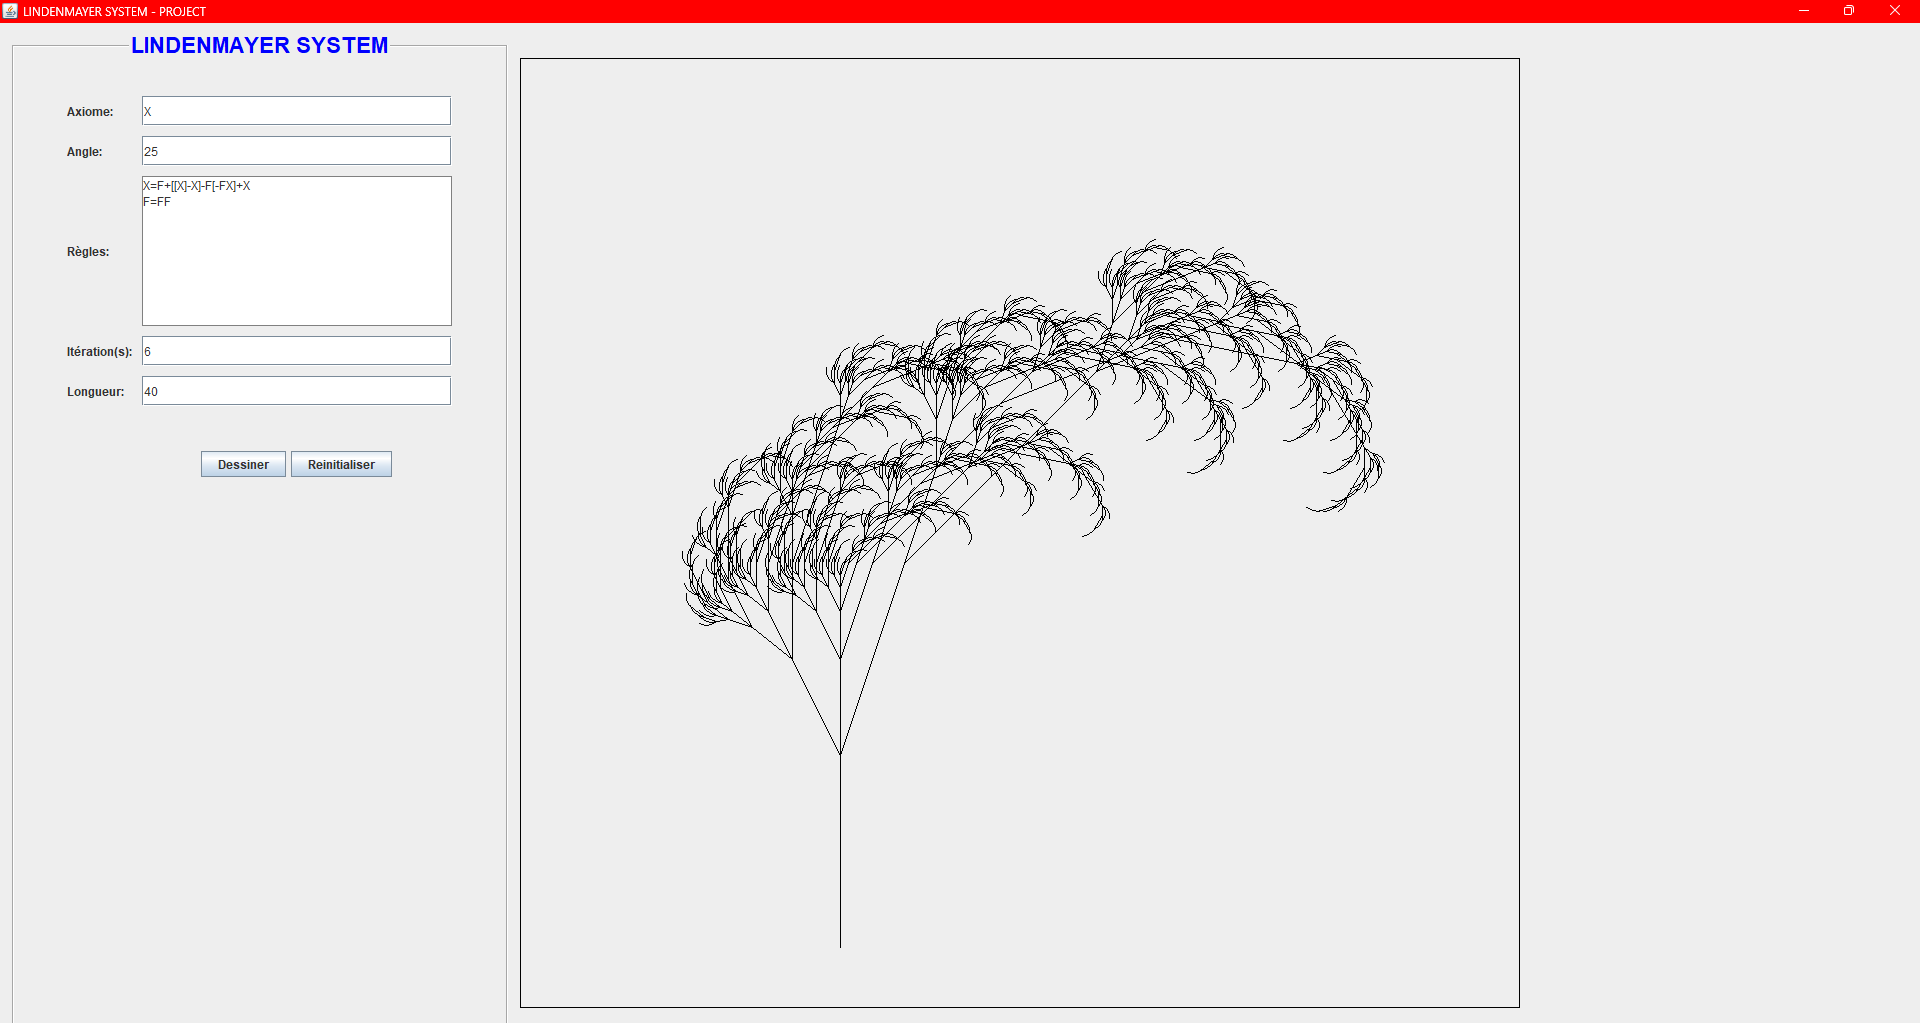
\includegraphics[width=0.49\textwidth]{./images/ArbreFractal.png}}
\hfill
\subfigure[Courbe de Koch]{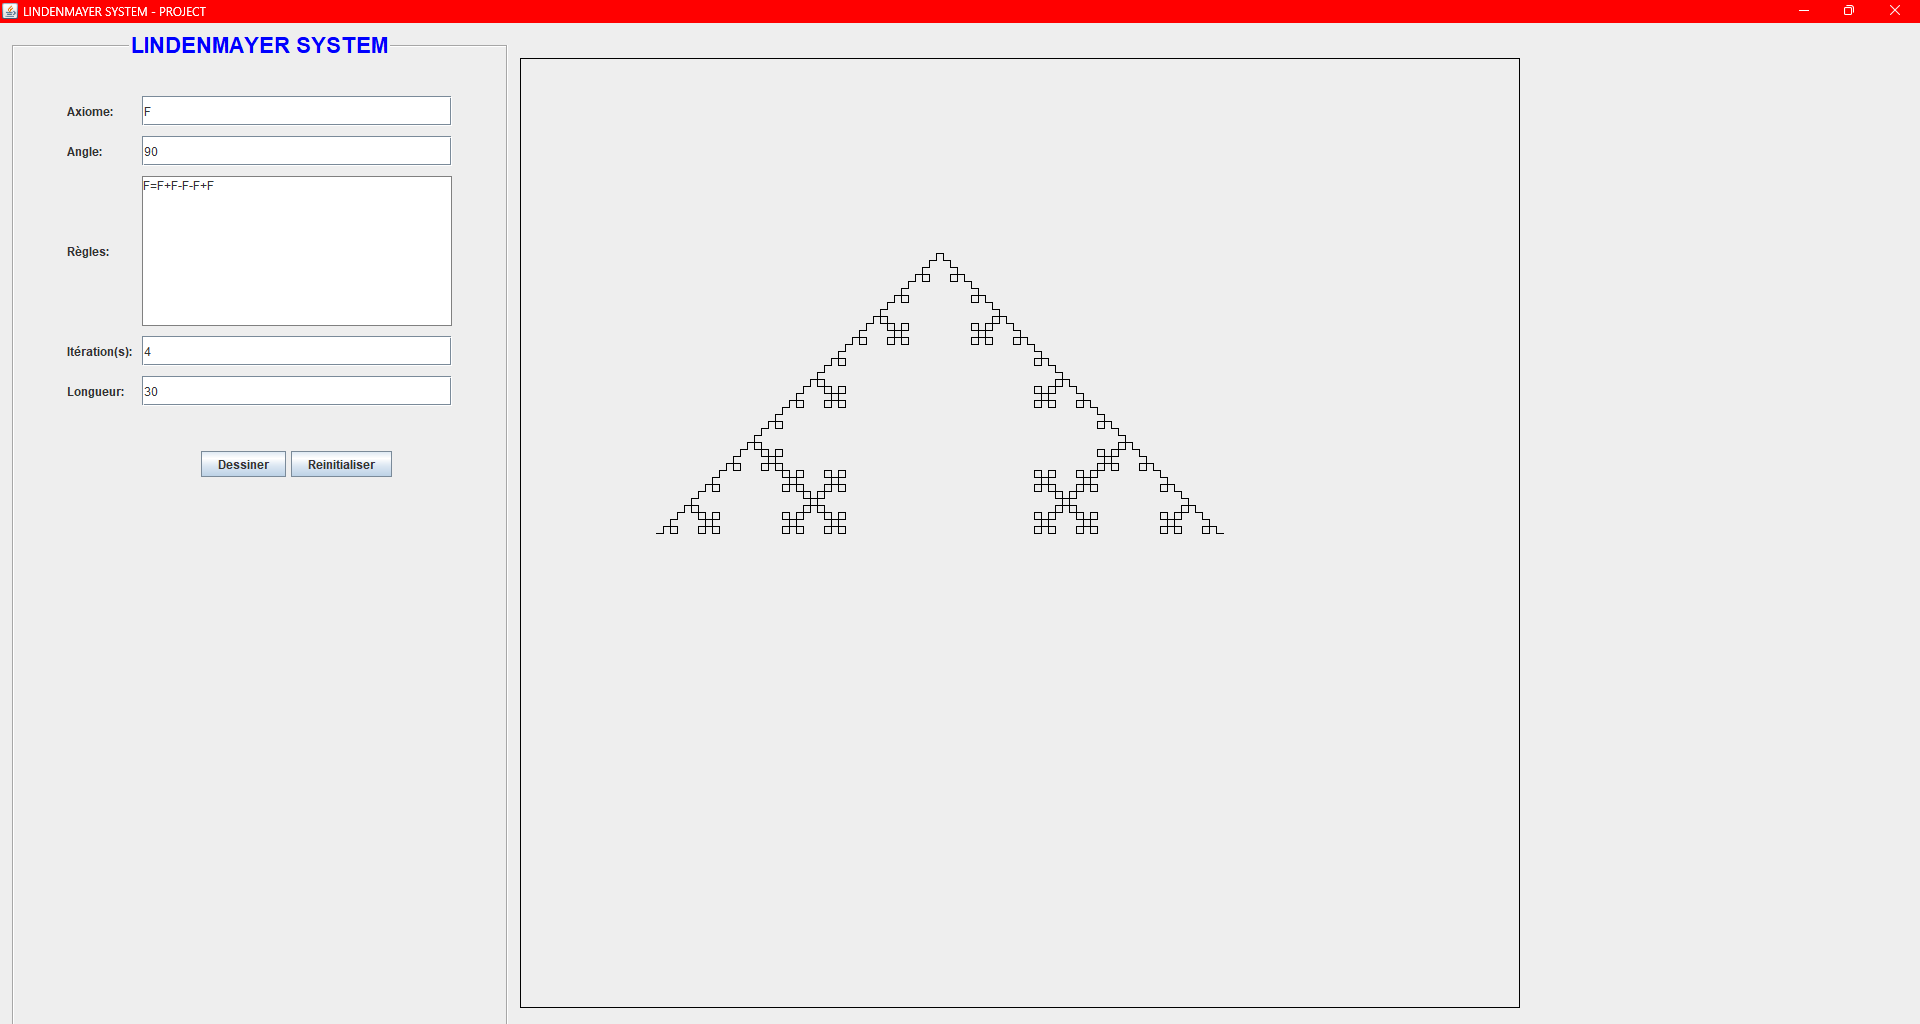
\includegraphics[width=0.49\textwidth]{./images/CourbeKoch.png}}
\caption{2 Exemples\label{fig:figure4}}
\end{figure}

\begin{figure}[h]
	\center
	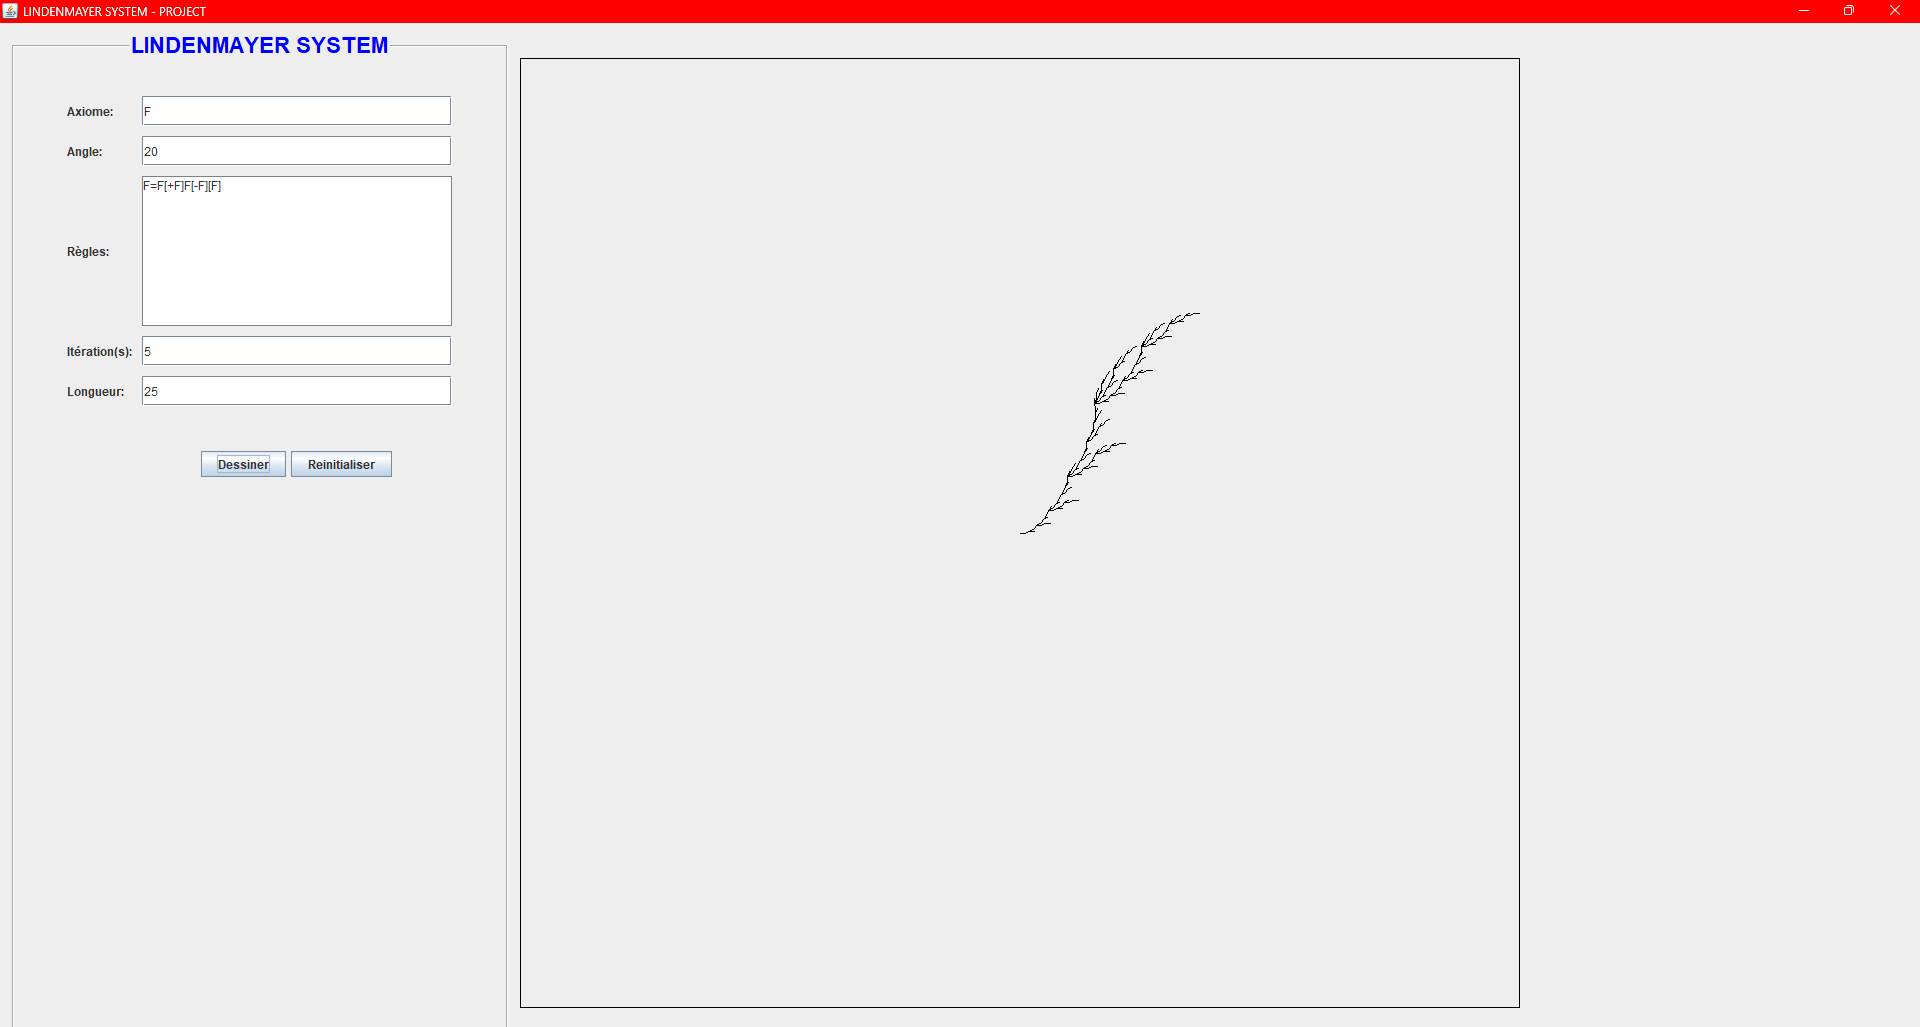
\includegraphics[width=0.49\textwidth]{./images/AutreArbre.png}
	\caption{Autre arbre en fractal \label{fig:figure5}}
\end{figure}
\newpage
Voici ci-dessus quelques exemples de cas d'utilisation.
Nous constatons que la figure \ref{fig:figure4}a et la figure \ref{fig:figure5} y font apparaître des représentations en deux dimensions de végétaux. Tandis que la figure \ref{fig:figure4}b nous montre un exemple plus mathématique et géométrique de la représentation d'interprétations graphiques.

Pour construire les dessins de la figure~\ref{fig:figure4} nous avons pris comme exemple, les axiomes fournis par la page Wikipédia anglais du LSystem que voici : \url{https://en.wikipedia.org/wiki/L-system#Example_4:_Koch_curve} et \url{https://en.wikipedia.org/wiki/L-system#Example_7:_Fractal_plant}. En ce qui concerne la figure \ref{fig:figure5} nous avons pris l'axiome fournis par le pdf qui se situe à l'url plus tôt évoquée dans le paragraphe \ref{lien:lien1}.


\section{Conclusion}
\subsection{Récapitulatif}
Dans ce projet nous avons pu implémenté un système de réécriture autonome qui peut être généré à partir d'une chaîne de caractères et qui est capable d'interpréter le résultat en dessinant. Nous avons pu par l'intermédiaire du besoin créer un Parser permettant la transformation d'une information en Objet.


\subsection{Propositions d'amélioration}
Bien que notre projet peut faire fonctionner les réécritures simples de LSystem. Nous n'avons pas abordé les différents mode de LSystem tel que le mode stochastique ou encore le mode contextuel qui existe. De plus notre logiciel pourrait être améliorer en rajoutant quelques boutons en plus pour permettre une meilleure ergonomie. Comme la translation d'une figure, son agrandissement ou encore sa rotation. De plus nous ne nous sommes pas aventurer dans la visualisation 3D du lsystem qui est une suite évidente à ce projet.



\end{document}
